\chapter{Programming Models}
\label{chapter:ProgrammingModels}
In this chapter general information about the asynchronous programming and the reactive programming models are introduced. This includes main use cases and general workflow. The asynchronous programming section includes an introduction to the async/await model~\cite{DOC:AsyncAwait}. The reactive programming section includes information about ReactiveX~\cite{WEB:ReactiveXMainPage} which is the corner stone for all Rx driven implementations.
\section{Asynchronous Programming}
\label{section:AsyncProgramming}
%\subsection{Introduction}
Asynchronous programming is a programming technique designed to handle a common problem that sometimes occur in synchronous programming. Synchronous programming will always block the execution until the previous line of code is handled. A synchronous program delegates the operative systems resources to finish a single operation in the program, before moving on to the next operation and so on. However, blocking the execution thread in general causes issues with scalability, latency as well as in general give a very bad user experience. Meaning synchronous programming isn't optimal for certain operations which requires long execution time. Especially if the operation itself spends most of its time waiting, such as database requests or I/O bound operations~\cite{VIDEO:AsyncConBack, WEB:AsyncAwaitTut}. Keep in mind that asynchronous programming for different programming languages usually follow relatively the same workflow, however the naming of operations may differ. In this paper the terminology used for asynchronous programming will follow the ones used in the .Net framework. 

Asynchronous programming as the name implies is designed to run operations asynchronously. In the asynchronous programming model, operations are divided into a set of tasks that performs the operation whenever the scheduler has resources which it can freely delegate to it. 
However, the task created will not block the main thread instead the main thread continues on with the next operation~\cite{WEB:AsyncAwaitTut, VIDEO:AsyncConBack, DOC:AsyncAwait}.
The task will have a reference to an awaiter that has information in regard to the task's current state. Eventually the asynchronous operation will finish, and the result will be available in the awaiter for the main thread to collect. Although tasks doesn't necessarily always return a physical result, nevertheless a task will always return an awaiter so that the main thread has all the information it requires for the running task~\cite{WEB:AsyncAwaitTut}.

Normally the program needs to receive the result of the asynchronous operation before reaching specific parts of the program that requires the result in order to run properly. Asynchronous functionality supports this functionality by allowing the designer to specify to the awaiter that the program is to wait at this point until the asynchronous operation is finished. This will still not block the main thread as the other tasks can be performed in the background unlike synchronous programming. Additionally, asynchronous programming has the benefit that the operation can be initialized earlier and be worked by the main thread while going through the operations to the point were the result is expected. This means asynchronous programming could avoid bottlenecks that occur in synchronous programming and thereby is more responsive of the two~\cite{DOC:TaskAsyncProgModel, WEB:AsyncAwaitTut}. 
For this reason, asynchronous programming has become the preferred programming model when it comes to designing user-interfaces. As it is important to avoid potentially blocking user input while another task is performed~\cites{VIDEO:AsyncConBack}[p.~214]{BOOK:DotnetMultithreadCookBook}. Server design is another example where asynchronous design is preferred as it handles large number of requests easier than a server with synchronous design~\cite{VIDEO:AsyncConBack, DOC:AsyncAwait}.

Asynchronous programming usually follows one or more of these three design patterns: 
\begin{itemize}
	\item{Asynchronous Programming Model(APM)}
	\item{Event-based Asynchronous pattern(EAP)}
	\item{Task-based Asynchronous Pattern (TAP)}
\end{itemize}
TAP is the most used design pattern and is the model used by the async/await workflow~\cite{DOC:AsyncAwait, WEB:AsyncAwaitTut}.

Asynchronous programming should not be confused with parallel programming as asynchronous methods do not create new threads. It instead runs on the current thread whenever the scheduler has resources ready and the operation itself is ready to progress. Therefore, the work required to create new threads as well as a lot of the work to keep the threads consistent can be omitted~\cite{DOC:TaskAsyncProgModel}. %Potentially write more once you have more control over how consistency works between async functions and how they fail in my implementation.

\subsection{Async/Await}
Asynchronous programming is not a new concept and C\# has long had support for it. However, before the async/await workflow became normalized programming asynchronously was quite difficult and even worse for others to read~\cite{DOC:TaskAsyncProgModel}. The workflow consisting of a lot of nested callback functions which is quite a struggle to manage properly. Today managing this kind of structure is referred to as \emph{callback hell}~\cites[p.~1-2]{PAPER:Callbackhell}[p~.2]{PAPER:PaxosCleipnir}. 

As mention previously the async/await workflow follows the TAP abstraction~\cite{DOC:TaskAsyncProgModel} meaning the workflow consist of creating asynchronous operations and then choose the point where we need the result of the asynchronous operation. The async/await workflow consist of three steps for the programmer. The first step is to assign the \code{async} modifier to a function to mark it as an asynchronous function. This allows asynchronous calls to be made inside the chosen function. The second step is to make an asynchronous call. Lastly specify the \code{await} operator for the awaiter for the asynchronous task~\cite{WEB:AsyncAwaitTut, DOC:AsyncAwait, VIDEO:AsyncConBack}.
 
Important to remember that the \code{await} operator can only be used in a function marked with the \code{async} modifier. In order to use asynchronous function call in a synchronous function the traditional operators have to be used instead\cite{DOC:AsyncAwait, DOC:TaskAsyncProgModel}. 

In \autoref{code:asyncawaitex} we can see a practical example of the async/await workflow.
The code in \autoref{code:asyncawaitex} is the function that is responsible for sending a message over the network. In order for the \code{SendMessage} to be marked as a asynchronous function it has \code{async} modifier. \code{SendMessage} does not return any values, therefore it returns a .Net \code{Task} object. Most of the code in the function is synchronous and this code transforms message object to byte streams. The last however is asynchronous where the socket object calls the asynchronous function \code{SendAsync}. As we want to avoid the function to return before the asynchronous operation is finished the \code{await} operator is used to wait for asynchronous operation to finish.
%TODO find/write a better example.
\begin{figure}[h]
	\centering
	%\lstset{style=sharpc}
	\begin{lstlisting}[label = code:asyncawaitex, caption=Example of async/await workflow, captionpos=b, basicstyle=\scriptsize]
public async Task SendMessage(byte[] sermessage, 
                              Socket sock, 
                              MessageType type)
{
    Console.WriteLine($"Sending: {type} message");
    var mesidentbytes = Serializer
                        .AddTypeIdentifierToBytes(sermessage, type);
    var fullbuffmes = NetworkFunctionality
                      .AddEndDelimiter(mesidentbytes);
    await sock.SendAsync(fullbuffmes, SocketFlags.None);
}


	\end{lstlisting}
\end{figure}
%\cite{VIDEO:AsyncConBack}
%\cite{DOC:AsyncAwait}
%\cite{DOC:TaskAsyncProgModel}
%\cite{BOOK:DotnetMultithreadCookBook}
%\cite{WEB:AsyncAwaitTut}
\section{Reactive Programming}
\label{section:reactive}
Reactive programming is a programming paradigm that focuses on changing the state of the program in response to some outward changes~\cite{WEB:RxProgIntro, DOC:Cleipnir}.
Reactive programming follows an event driven workflow. An event can be triggered from one part of the system and when this event is received by the other part it starts altering the state of the system in response. Reactive programming works hand in hand with asynchronous event-based programming which was mentioned previously briefly in \autoref{section:AsyncProgramming}~\cite[p.~2-3]{BOOK:RxLinq}. Reactive programming is commonly used to handle a continuous stream of asynchronous data~\cite{VIDEO:dotnetsheffReactive}. 
Currently there exists a lot of support for Reactive programming. Specifically, the library Reactive X~\cite{WEB:ReactiveXMainPage} has presented a general \ac{api}~\cite{web:api} for implementing the core concepts of reactive programming. As a result, today there exist a lot of reactive extensions for multiple programming languages. Rx.Net~\cite{Github:ReactiveExtensions} is the official .Net reactive extension. Cleipnirs has implemented its own reactive extension that resembles Rx.Net very closely. The main difference between the two is that Cleipnirs reactive layer supports persistency, but lacks reactive operators that Rx.Net does support~\cite{DOC:Cleipnir}.
Although Cleipnir and Rx.Net vary somewhat from the general \ac{api}, the general workflow remains the same. Therefore we will introduce the main concepts of Reactive X in this section. Details specific for Cleipnir are instead presented in the upcoming \autoref{chapter:Cleipnir}.

\subsection{Reactive X}
ReactiveXs workflow can be easily summarized with the following tasks~\cite{WEB:ReactiveObservable}
\begin{enumerate}
	\item{Start an asynchronous operation that will perform some work and eventually return it}
	\item{Transform the asynchronous operation as an Observable object}
	\item{Use reactive operators to transform/filter the resulting data.}
	\item{Observers subscribe to the Observable and waits for the Observable to return the data}
\end{enumerate}

An observable object follows a similar structure to an enumerable object, where the main difference between an enumerable and an observable object is their method of accessibility. In an enumerable object will give the next object in storage whenever asked for it. In other words, the program will dictate when the next entry will be collected. In an Observable object the next result is instead pushed to its subscriber whenever the result is ready. The program has no control over when the next entry will be ready as it is waiting for an asynchronous operation to complete~\cites{WEB:ReactiveObservable, VIDEO:dotnetsheffReactive, VIDEO:MicroDev}[p.~15]{BOOK:RxLinq}. Observables, like enumerable, support the use of \ac{linq} queries on its resulting data. \ac{linq} add additional operators for filtering and transforming the resulting data into new enumerables~\cites{VIDEO:dotnetsheffReactive}[p.~3-4]{BOOK:RxLinq}[p.~208]{BOOK:DotnetMultithreadCookBook}.

Traditionally, the implementation is expected to incorporate the following functions for its observer object.
\begin{itemize}
	\item{OnNext}
	\item{OnError}
	\item{OnCompleted}
\end{itemize}

OnNext is the function that handles each new incoming event emitted by the Observable. OnError is the function that is called if an error occurs within handling one of the emitted events. OnCompleted is the function that is called when the observable is finished and will no longer emit any new events~\cite{WEB:ReactiveObservable}.

In some implementations the Observable and observer functionality are merged together into an object called subject. A subject object acts as a bridge of sorts between the observer and the observable where its main usage is to simplify the workflow for reactive programming. A subject has the ability to subscribe to an observable just like an observer. However, unlike an observer a subject can also re-emit events already processed in the observable, as well as be used for emitting new events to the observable. Eventually, all the items emitted by the subject will also be handled by the subject, making the programming workflow a lot simpler compared to its traditional style~\cite{WEB:ReactiveSubject}. Cleipnir supports subject in its implementation, however the objects are not referred to as subject, but rather source objects.

\iffalse
-a brief introduce reactive programming
-usecase
-the ReactiveX library(what it does, how it works and the mention Rx.Net)
-give brief through workflow, concepts with name and definitions and how it works.(Observable, stream of data, subjects, event driven programming)
-mention briefly Cleipnir support for reactive programming, how they differ, say detail information is given in Cleipnir chapter.
\fi


%\chapter{Practical Byzantine Fault Tolerance}
\label{chapter:PBFT}
%version 1
This chapter presents the Practical Byzantine Fault tolerance(PBFT) consensus algorithm in detail.
Starting with introducing the system model commonly used for PBFT. Then a detailed explanation is given for how the protocol normally operates. This includes mechanisms such as checkpoint and leader changes.

\section{Introducing Practical Byzantine Fault Tolerance}
Practical Byzantine Fault Tolerance(PBFT) is a consensus algorithm specifically designed to handle Byzantine faults in an asynchronous distributed network. The algorithm was originally published in 1999 by Miguel Castro and Barbara Liskov~\cite{PAPER:OGPBFT}.
Notably the Linux foundation's open source blockchain by the name of Hyperledger~\cite{WEB:PBFTGeeks, SLIDES:PBFT} uses PBFT.

The problems derived from byzantine faults originally came to light through a well-known problem known as the Byzantine Generals Problem~\cites{WEB:BFTInfo}{ART:lamportByzGenProb}[p.~240-253]{BOOK:BuildDepDistSyst}.
The byzantine generals' problem can be summarized as a couple of army generals which are each leading their own armies and they need to together reach a decision. The most common scenario used is  that the armies try to coordinate an attack on a surrounded city. The armies can only survive if the majority of the generals agree to either attack the city together or majority agree to retreat to fight another day. There are also traitor generals that actively attempt to sabotage the order. The decision is also irreversible regardless of the action performed by the other armies. A byzantine fault tolerant system is a system that can handle the issue introduced by the byzantine generals problem and is the main goal for consensus algorithms to achieve this state. This includes the PBFT algorithm~\cite{WEB:BFTInfo, ART:lamportByzGenProb}.

The PBFT algorithm focuses on creating a state machine network that can withstand byzantine failures~\cite[p.~456]{BOOK:MVstandver3}. The protocol achieves this by providing the network with two main properties. These properties are referred to as safety and liveness.
To summarize these properties:\\
\textbf{Safety} is the property that ensures that the total ordering of requests is equal for all the non-faulty participating servers. In other words the system state should be similar to a synchronous system, operating one operation at the time, despite the fact that the system is operated over multiple remote machines.\\
\textbf{Liveness} is the property that ensures that the correct result is eventually agreed upon and returned by the system~\cites[p.~456]{BOOK:MVstandver3}{WEB:ConsesAlgo}[p.~2]{PAPER:OGPBFT}{SLIDES:PBFT}[p.~403]{PAPER:PBFTRecovery}[p.~257]{BOOK:BuildDepDistSyst}.

\section{System Model}
\label{section:systemModel}
The PBFT consensus algorithm is implemented using \emph{R} number of servers referred to as \emph{replicas}. When a replica is down or behaving maliciously then we say that the replica is faulty. The number of faulty replicas is symbolized as \emph{f}. 
Quorum is a term used to refer to the limit of messages required to verify that the majority of replicas in the system agreed upon a decision\cites[p.~408-409]{PAPER:PBFTRecovery}. %Add another more detailed cite here!
A single replica is chosen as the leader called primary, and is represented as \emph{p}. The other replicas are referred to as backups. The responsibility of the primary is to order the request sent to the system by numerous clients~\cites[p.~456]{BOOK:MVstandver3}[p.~405]{PAPER:PBFTRecovery}. The replica that is chosen as the primary is based on the replica's identifier value.

According to~\cites[p.~3]{PAPER:OGPBFT}[p.~405]{PAPER:PBFTRecovery}, replicas in the distributed network move through "successions of configurations known as views". A simpler definition for a view is a number that defines the set of non-faulty replicas that are participating in the current PBFT protocol round set up by the current primary. The current view number is symbolized by \emph{v}.
As mention previous the primary is chosen based on an identifier value emph{i}. That identifier value determined by the formula $p = v mod R$~\cites[p.~258]{BOOK:BuildDepDistSyst}[p.~3]{PAPER:OGPBFT} {SLIDES:PBFT}. 
We decided to set the initial view number to zero, which results in the formula setting replica zero as the initial primary.

The protocol can only guarantee the safety and liveness properties of a system if the number of faulty replicas does not exceed a specified margin of the total replicas in the network. The total number of replicas required to be in the system should be derived by the formula $R > 3f + 1$.
The formula shows potentially that for each new faulty replica that is to be handled in the network, additional three servers are required. As an example, the lowest number of replicas a system can have is four. In this situation their system can only handle 1 faulty replica. In order to handle more faulty replicas the system has to scale up by adding three additional servers for each faulty server that exist\cites[p.~257]{BOOK:BuildDepDistSyst}[p.~403]{PAPER:PBFTRecovery}{SLIDES:PBFT}[p.~3]{PAPER:OGPBFT}.

All the messages sent between replicas are expected to be digitally signed by their sender. The signature process uses public-key cryptography~\cite[p.~257,p.267]{BOOK:BuildDepDistSyst}. A hidden private key is used to sign the messages while the other parties can use the replicas public key to verify this signature~\cite[p.~417]{PAPER:PBFTRecovery}. The signature procedure is used to verify that the sender are who they claim to be~\cite[p.~3]{PAPER:OGPBFT}. In some cases, the digital signatures are replaced with a Message Authentication Code (MAC). This is done for removing potential bottlenecks in performance as well as to detect tampering\cites[p.~257]{BOOK:BuildDepDistSyst}[p.~3,8]{PAPER:OGPBFT}. In this PBFT implementation, digital signatures are used for all message types.


%According to~\cite{PAPER:OGPBFT,PAPER:PBFTRecovery} page 3 and 8 respectively, replicas move through "successions of configurations known as views". A simpler definition for a view is a number that defines the set of non-faulty replicas that are participating in the current PBFT protocol round set up by the current primary. , where p refers to the primary, v is the current view number and |R| is the number of replicas.

\section{Detailed Protocol Operations}
\label{sec:detailedProtocol}
The PBFT consensus protocol is divided into three phases. The Pre-Prepare, Prepare and the Commit phase. If the PBFT protocol operations are executed properly, consensus has been achieved for an operation once all three phases have transpired on $3f+1$ replicas~\cite[p.~257-259]{BOOK:BuildDepDistSyst}. Role of the pre-prepare phase and prepare phase is to propose an ordering for requests delivered to the system, while the combination of prepare phase and the commit phase establishes the execution order for the replicas in the system~\cite[p.~4]{PAPER:OGPBFT}. \autoref{fig:pbftnormalworkflow} shows an illustration of the PBFT workflow. The illustration shows the messages sent from the different replicas during the different protocol phases in PBFT.

The PBFT protocol starts once a client sends a request containing their desired operation to the primary~\cite[p.~4]{PAPER:OGPBFT}. Sometimes the client will also multicast their request to the other replicas in the system as well, which is the model that we followed in our implementation~\cites[p.~2]{PAPER:DPBFT}[p.~406]{PAPER:PBFTRecovery}[p.~258]{BOOK:BuildDepDistSyst}. Regardless of which of these models is used for the request message, the primary is the one responsible for starting the iteration of the PBFT algorithm to process the client's request. The primary will create a Pre-Prepare message and assign the request with a sequence number which is then multicasted to the other replicas in the network that have the same view number as the primary. Once a replica receives the Pre-Prepare message it will validate the Pre-Prepare message. The validation process consist of the following~\cites[p.~4]{PAPER:OGPBFT} {SLIDES:PBFT}[p.~259]{BOOK:BuildDepDistSyst}
\begin{itemize}
	\item[-]Validating the Signature in the message.
	\item[-]Checking that the view number in the message matches the current view number.
	\item[-]The message sequence number is not out of bounds with the current sequence number interval~\cites{SLIDES:PBFT}[p.~4]{PAPER:OGPBFT}.
	\item[-]Make sure the replica has not already received another Pre-Prepare message with the same sequence number, but with a different request.
\end{itemize}
Once the validation process is finished the replica officially starts the prepare phase by creating a prepare message and multicasting it over the network. The prepare phase ends for a replica once it's stored up to $2f+1$ validated pre-prepare/prepare messages from different replicas. After this condition is met, the replica enters the state known as \emph{prepared}. In this state it will log the message data thus far in what is called a \emph{prepare certificate}. A prepare certificate is essentially a record that shows that the prepared phase is finished and is properly executed for that given request. The proof provided in a prepare certificate is a list of the valid prepare messages, basically confirming that quorum has been reached for the certificate when the number of messages stored in the list is higher than the desired limit of $2f + 1$~\cites[p.~408]{PAPER:PBFTRecovery}[p.~457]{BOOK:MVstandver3}.
The last phase is the commit phase which functions very similar to the prepare phase. Each replica that is finished with the prepare phase will start the commit phase by multicasting commit messages to the other replicas in the system~\cite[p.~4]{PAPER:OGPBFT}. In this phase, the primary functions exactly the same as every other replica. The validation process is also the same as it was for prepare messages. The goal for the commit phase is also the same as in the prepare phase, which is for a replica to receive $2f+1$ commit messages, which includes the replica's own commit message~\cite[p.~5]{PAPER:OGPBFT}. Once a replica has received enough commit messages, then the protocol reaches the \emph{committed} phase for the replica. This essentially means that a commit certificate is created and is logged similar to a prepare certificate~\cites[p.~409]{PAPER:PBFTRecovery}[p.~457]{BOOK:MVstandver3}. When a replica has finished both a prepare certificate and a commit certificate, then consensus has been achieved and each replica will perform the operation requested by the client~\cites[p.~409]{PAPER:PBFTRecovery}[p.~5]{PAPER:OGPBFT}. After the operation is executed each replica sends back a reply message containing the appropriate identification values as well as the result of processing the given request. The last requests sent by the clients are also stored in memory, to account for the situation where the client does not receive the reply messages. In this case the client will re-transmit the same request to the system and the replicas will re-transmit their reply for that following request~\cite[p.~409]{PAPER:PBFTRecovery}. A client will accept the result if it gets $f+1$ replies back from the replicas.
 

The replicas can only handle a certain amount of requests before the system is required to save its state. As mentioned in the validation process, a replica can only process a protocol message that is within a given sequence number interval. This sequence interval length is always constant and will adjust based on the systems checkpoint period which will be discussed in the next section \autoref{sec:checkpoint}\cites[p.~262]{BOOK:BuildDepDistSyst}[p.~4-5]{PAPER:OGPBFT}.

\begin{figure}[!h]
	\centering
	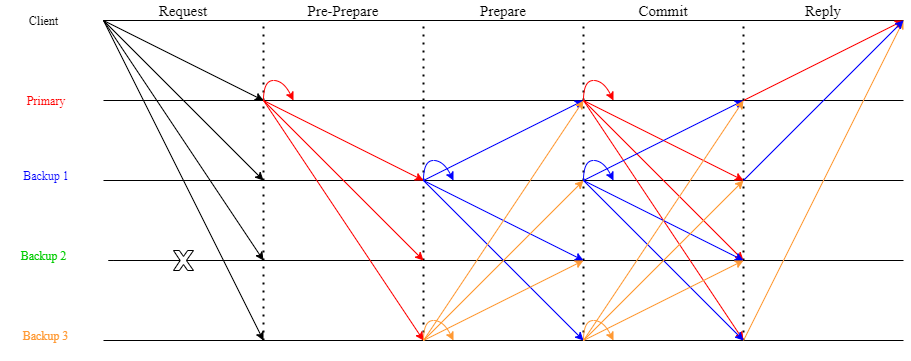
\includegraphics[width=\linewidth]{figures/PBFTWorkflow}
	\caption{Practical Byzantine Fault Tolerance Normal Workflow}
	\label{fig:pbftnormalworkflow}
\end{figure}

\section{Checkpointing}
\label{sec:checkpoint}
PBFT also incorporates checkpointing, which is a mechanism used for garbage collecting the logs. Checkpointing is required so that the replica does not use up all of its memory for logging messages~\cite[p.~261]{BOOK:BuildDepDistSyst}. Therefore, the replicas must agree upon a point in which the system is stable for all the replicas. Afterwards the replicas can delete any records in the logs prior to the consented state~\cites[p.~5]{PAPER:OGPBFT}[p.~410]{PAPER:PBFTRecovery}.

Checkpoints are essentially the state records of the system after progressing a specific interval of requests. The checkpoint has information regarding the last sequence number that was performed for the system. This sequence number is used on the garbage collector to put an upper bound on the records that are to be removed. For instance, if the stable sequence number was set to 50, then the garbage collector would remove a set of logged data up to 50. The checkpoint also has a digest of the system for that stable sequence number. This digest is used to confirm that the replicas have the same system state for the given sequence number~\cites[p.~5]{PAPER:OGPBFT}[p.~410]{PAPER:PBFTRecovery}.

In order for replicas to be able to validate checkpoints, they each must multicast a checkpoint message over the network containing the information mentioned above with its own replica id. Like the rest of the PBFT protocol messages a checkpoint is considered to be valid for a replica if it has stored $2f+1$ checkpoint messages with different replica id`s with the same stable sequence number and system digest~\cites[p.~261-262]{BOOK:BuildDepDistSyst}[p.~5]{PAPER:OGPBFT}[p.~410]{PAPER:PBFTRecovery}. Once a checkpoint has been validated successfully it is referred to as a stable checkpoint~\cites[p.~3]{PAPER:DPBFT}[p.~261]{BOOK:BuildDepDistSyst}. The replical usually stores checkpoint messages for different sequence numbers in memory and has only a single record for a stable checkpoint. Once a new stable checkpoint is determined, any checkpoint records with lower sequence numbers are removed from memory and if there exists a previous stable checkpoint in memory with a lower sequence number, then it is replaced by  the new one~\cite[p.~261-262]{BOOK:BuildDepDistSyst}.

In PBFT checkpointing is usually performed periodically after a constant number of requests have been processed. This interval length is constant and is referred to as a checkpoint period~\cites[p.~261]{BOOK:BuildDepDistSyst}[p.~410]{PAPER:PBFTRecovery}. As mentioned earlier in~\autoref{sec:detailedProtocol} PBFT normally only processes a sequence number if it is in the set of currently available sequence numbers. The length of the sequence number interval is usually designed to follow the format $[checkpointinterval+1-2*checkpointinterval]$. Which means the system attempts to calculate two checkpoints during a single sequence number interval. Once a stable checkpoint is obtained, the system extends the sequence number interval where the new interval starts at the last stable sequence for the current stable checkpoint~\cites[p.~5]{PAPER:OGPBFT}[p.~410]{PAPER:PBFTRecovery}. Unless a replica has exceeded the upper bound of the sequence number interval, the replical usually performs the checkpoint functionality concurrently to the protocol workflow.

\section{View-change}
\label{sec:view-change}
In the scenario in which the primary is the faulty replica, a view-change eventually occurs. The purpose of the view-change is to reassign the responsibility for a primary away from the current primary replica that is deemed to be faulty. Which is then given to another replica that is not faulty~\cites[p.262]{BOOK:BuildDepDistSyst}. As mentioned in \autoref{sec:systemModel}, the replica that is chosen as the next primary is based on the replica id and the next view number. Therefore, the view-change updates the view number for the system in order to change the primary replica of the system. There are some operations that need to be performed for a view-change to be deemed successful. The first operation is to update the view number to set another replica as the primary~\cites[p.~6]{PAPER:OGPBFT}[p.~411]{PAPER:PBFTRecovery}{WEB:SawtoothPBFT}. This step includes multicasting view-change messages between replicas to start the new view session. The other more demanding operation is that the primary needs to make sure that the system is stable and that replicas start the new view with the exact same system state. Therefore, all requests that have been performed after the last stable sequence number, need to be reprocessed between the replicas. This is done so that the system can guarantee that the replicas are not missing any of the previous operations performed to the system.~\cites[p.~458]{BOOK:MVstandver3}[p.~263-265]{BOOK:BuildDepDistSyst}.

There are several ways for a replica to deem its primary to be faulty, the most common way is to have a timeout functionality for the protocol execution. It is most common to start a timeout once a replica has received a request from the client. If the replica does not receive any pre-prepare messages for that request before the timeout expires, than the replica goes into view-change mode and no longer participates in any of the protocol operations~\cites{SLIDES:PBFT}[p.~5-6]{PAPER:OGPBFT}[p.~263]{BOOK:BuildDepDistSyst}.  

The view-change process starts by having the replica increment its view number. Then the replica creates, signesand multicasts a view-change message over the network. The replica  then waits for $2f+1$ view-change messages~\cites{SLIDES:PBFT}[p.~6]{PAPER:OGPBFT}[p.~411]{PAPER:PBFTRecovery}{WEB:SawtoothPBFT}. A timeout is also used here, if the replica does not receive enough view-change messages in time, then the process repeats with the next incremental view number. In some cases a replica can also be designed to go into view-change mode if a replica has already received two view-change messages from other replicas, as it now only requires its own view-change message for the system to agree that a view-change is necessary\cite{BOOK:BuildDepDistSyst}. Once the appropriate number of view-change messages are received, then the new primary is responsible for creating, signing and multicasting a new-view message to the other replicas~\cite[p.~264]{BOOK:BuildDepDistSyst}. Before the new-view message can be multicast to the other replicas, a new primary must go through its log and create new pre-prepare messages for all sequence numbers that have occurred after the last stable sequence number. If the new primary lacks a record in the log for any of the sequence numbers, the new pre-prepare message has its request digest be set to be \code{null}. This information is included in the new-view message, which is then sent to the other backup replicas. The backup replicas then validates and re-process each of the sequence numbers that have a valid pre-prepare message. This essentially means that the other replicas have to multicast a new prepare message and then participate in a commit phase together with the new primary for each of the pre-prepare messages in the new-view message~\cites[p.~6]{PAPER:OGPBFT}[p.~458]{BOOK:MVstandver3}[p.~265]{BOOK:BuildDepDistSyst}. A timeout is once again being used to handle the situation where the reprocessing takes too long. This process can also fail if the pre-prepares in the new-view message fails the validation process. If either the timeout occurs or the validation fails, then it is back to the start for the view-change process. Once all pre-prepares have been reprocessed, the view-change procedure is over, and the replica returns to normal protocol operations with the new chosen primary. Keep in mind that any new requests received during the view-change process are ignored by the system~\cite[p.~263]{BOOK:BuildDepDistSyst}. 

\autoref{fig:pbftviewchange} shows an example of a view-change process. The figure shows the timeline for each of the processes needed for the view-change to be successfully completed. Starting with the timeout occurring on the backup replicas when the primary is no longer working properly. Then the replicas each multicast a view-change message to the other replicas in the system, including the faulty primary. After the new primary has received a sufficient number of view-change messages, it creates pre-prepares messages that need to be reprocessed in the network. Afterwards the new primary multicast new-view messages to the other replicas to start the re-processing phase. Finally the system multicasts both prepare and commit messages to validate pre-prepare messages. Once all that is done the system moves on to normal workflow again with the first backup replica now serving as the primary for the system.

\begin{figure}[!h]
	\centering
	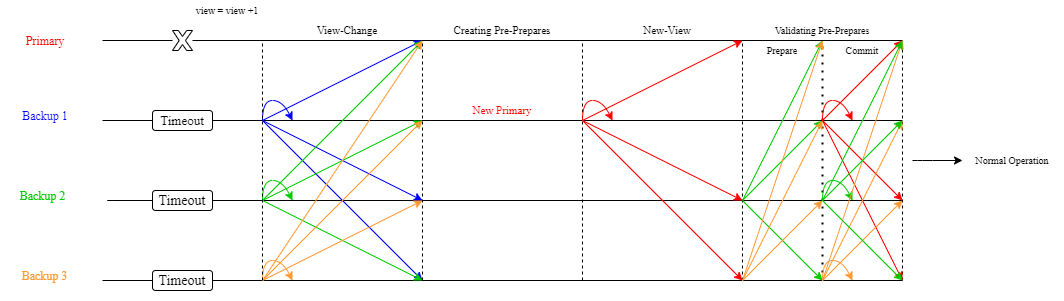
\includegraphics[width=1.1\textwidth]{figures/PBFTViewChange}
	\caption{Practical Byzantine Fault Tolerance View-Change}
	\label{fig:pbftviewchange}
\end{figure}

%In the scenario in which the primary is the fault replica, a view-change occurs. The purpose of the view-change is to reassign the primary responsibility away from a replica that is deemed to be faulty. As mentioned in \autoref{sec:systemModel}, the replica which is chosen as the primary is based on the replica id and the current view number. Therefore, the view-change updates the view number to update the primary replica. There are 3 main operations that need to be performed for a view-change to be deemed successful. The first is to update the view number to set another replica as the primary. The second is to validate this new leader on whether it is a suitable replacement. Finally, all operations that are performed after the last stable checkpoint needs to be reprocessed between the replicas. There are several ways for a replica to deem its primary to be faulty, the most common way is to have a timeout functionality for the protocol execution. The one that is most common is to start a timeout once a replica has received a request from the client. If the replica does not receive any pre-prepare messages for that request before the timeout expires, the replica will go into the view-change mode and will no longer participate in any of the protocol operations.  

%The view-change process starts by having the replica increment its view number. Then the replica will create, sign and multicast a view-change message. The replica will then wait for $2f+1$ view-change messages. A timeout is also used here, if the replica does not receive enough view-change messages in time, then the process repeats with the next incremented view number. In some cases a replica can also be designed to go into view-change mode if a replica has already received two view-change messages from other replicas, as it now only requires its own view-change message for the system to agree upon the view-change. Once the appropriate number of view-change messages are received, then the new primary will be responsible for creating, signing and multicasting a new-view message to the other replicas. Before the new-view message can be multicast to the other replicas, a new primary must go through its log and create new pre-prepares for all sequence number that has occurred after the last stable sequence number. If the new primary lacks a record in the log for any of the sequence numbers, the new pre-prepare message will have its request digest be set to null. This information is included in the new-view message, which is then used by the other replicas to validate and re-process each of the sequence numbers that has a valid pre-prepare. This essentially means that the other replicas have to multicast a new prepare message and then participate in a commit phase together with the new primary for of the pre-prepare messages in the new-view message. A timeout is once again being used in the case where the reprocessing fails or takes too long. This process can also fail if the pre-prepares in the new-view message fails the validation process. If this happens, then its back to start and in the view-change process. Once all pre-prepares have been reprocessed, the view-change procedure is over, and the replica will return to normal protocol operations using the chosen new primary. Any requests received during the view-change process will be ignored by the system. 

%TODO rewrite after implementing the basics of view change for app
%In the scenario where the primary is the faulty replica a view change occurs. A view change increments the view number for all participating replicas, which in turn chooses as a new primary replica for the network following the formula mention in \autoref{section:systemModel}. 
%Normally each replica starts a timeout operation whenever it receives a request from a client~\cite[p.~415]{PAPER:PBFTRecovery}. 
%If the replica does not receive a pre-prepare message before the timeout expires, then the replica deems the primary to be faulty and desires a view change. The replica will multicast a view-change message to the other replicas in the view, including the potentially faulty primary, and will ignore any %new incoming messages with the exception of view-change, new view and checkpoint messages~\cites[p.~5-6]{PAPER:OGPBFT}[p.~263]{BOOK:BuildDepDistSyst}. 
%A replica receiving a view change will reply with a view-change-ack.  The new primary chosen will collect view-change messages and view-change-ack messages to create a view-change certificate. Once the certificate is valid and has reached $2f+1$ unique messages a new-view message is multicasted to %every replica in the network, officially starting the new view~\cites[p.~412-414]{PAPER:PBFTRecovery}[p.~263-p.265]{BOOK:BuildDepDistSyst}[p.~458]{BOOK:MVstandver3}.
%%PBFT also incorporates checkpointing, which is a mechanism used for garbage collecting the saved logs. Without checkpoints, the replica would eventually use up all of its memory for logging protocol messages~\cite{BOOK:BuildDepDistSyst}. 
%%Checkpoints are essentially a proof where the replicas have agreed on a stable state for the system after a specified interval of requests has been processed~\cite[p.~5]{PAPER:OGPBFT}. For instance, if the checkpoint interval was set to 50, then the system would only allow sequence numbers 0 to 50 to %be performed in the first interval. Once the checkpoint interval is reached the log data is hashed and saved as a checkpoint message. The message is then multicasted over the network. Consensus is reached when a replica receives $2f+1$ checkpoint messages with different identifiers, but they all have same checkpoint hash value. The checkpoint is then saved on the replica and all the protocol messages with lower or equal sequence number to the checkpoint interval will be deleted from the log. As an example, if the checkpoint interval was 50, then certificates saved up for requests 0 to 50 are deleted. Then the interval is updated to be $[checkpointinterval+1-2*checkpointinterval]$, so for the last example the new interval would be between 51 to 100~\cites[p.~3]{PAPER:DPBFT}[p.~5]{PAPER:OGPBFT}[p.~409-410]{PAPER:PBFTRecovery}[p.~p.261-262]{BOOK:BuildDepDistSyst}.

\iffalse
\cite[p.~415]{PAPER:PBFTRecovery}
\cite[p.~5-6]{PAPER:OGPBFT}
\cite[p.~263]{BOOK:BuildDepDistSyst}
\cites[p.~3]{PAPER:DPBFT}
\cite[p.~458]{BOOK:MVstandver3}
\fi

%\cite{WEB:PBFTGeeks}
%\cite{WEB:ImpPBFTBlock} %not used
%\cite{WEB:UnderpBFT} %not used
%\cite{WEB:PBFTConSeries} %not used
%\cite{SLIDES:PBFT}
%\cite{VIDEO:YPBFT}
%\cite{BOOK:MVstandver3}
%\cite{BOOK:BuildDepDistSyst}
%\cite{PAPER:OGPBFT}
%\cite{PAPER:DPBFT}
%\cite{PAPER:PBFTRecovery}
%\lstset{style=sharpc}
%\begin{lstlisting}
%Your c# code here
%class Request
%{
%	private m string;
%} 
%\end{lstlisting}
